\section{Data Modelling}
Coming up with a domain model is a process which can provide clarity and direction for a software system, even on a small scale such as in a library. 

\subsection{Intermediate Features}
Common for many of the algorithms for finding user mobility features is that they rely on clustering of data points, to reduce the initial amount of data points into clusters representing locations where the participant did not move around a lot. For spatial clustering such as 2D data points on the surface of the earth, many of the algorithms use the DBSCAN algorithm as discussed in Chapter \ref{chapter:02-related-work}. The modelling approach is loosely based on the \cite{sparse-location-2014} a basic modelling approach for pre-processing is provided, which will be used for this thesis. The pre-processing produces \textit{intermediate features} from which the final mobility features are derived. These intermediate features are \textit{Stops}, \textit{Places} and \textit{Moves} and provide a course-grained version of the dataset which makes the final feature calculation much cheaper, computationally speaking. We define \textit{Places} as specific locations of relevance to the user, such as home or workplace. \textit{Stops} are specific visits to any of those places. Thus, a \textit{Stop} is always associated with a single \textit{Place} while places can be associated with one or more \textit{Stops}. Finally, \textit{Moves} are the sequences of location samples in between \textit{Stops}, representing moving between \textit{Places}. 

\subsection{Data Model Overview}
In order to capture the data model in an object-oriented programming language, a UML diagram was maintained as the implementation went along in order to keep track of relationships between the classes. 
% As a general rule of thumb, all the fields were made public including those required by the constructors, and the methods of the classes were all \textit{getters}, i.e. \\

\subsubsection*{Location}
A \textit{Location} is defined by a geographical \textit{latitude} and \textit{longitude} and represents a real-life location.

\subsubsection*{Cluster}
A \textit{Cluster} is created from a collection of \textit{Locations}. This class serves as an auxiliary class for clustering based on median \textit{latitude} and \textit{longitude}.

\subsubsection*{Single Location Point (SLP)}
A \textit{Single Location Data Point} (SLP) is a time-stamped \textit{Location}. By having a time-stamp, a collection of SLPs may be ordered and grouped by the time of day. In essense, the SLP is a Data Transfer Object (DTO) \footnote{\url{https://martinfowler.com/eaaCatalog/dataTransferObject.html}} which is used to transfer GPS data from an arbitrary Location plugin to the \textit{Mobility Features Package}.

\subsubsection*{Hour Matrix}
An \textit{Hour Matrix} is a matrix with 24 rows and columns equal to the number of places of some period. The \textit{Hour Matrix} class is used to calculate the \textit{Routine Index} feature, as well as to identify the \textit{Home Cluster}, which is the place most visited during 00:00 and 06:00. An Hour Matrix is constructed from a list of \textit{Stops} which all have the same date.

\subsubsection*{Stop}
A \textit{Stop} is a visit at a known \texit{Place} (see below) for an extended period of time. A \textit{Stop} is defined by a location which represents the centroid of a collection of data points, from which a \textit{Stop} is created. In addition a \textit{Stop} also has an \textit{arrival}- and a \textit{departure} time-stamp, representing when the user arrived at the place and when the user left the place. From the arrival- and departure timestamps of the \textit{Stop} the duration can be computed.

\subsubsection*{Place}
A \textit{Place} defined as a group of stops which were clustered by the DBSCAN algorithm \cite{density-based-1996}. From the cluster of stops, the centroid of the stops can be found, i.e. the center location. In addition, it can be computed how long a user has visited a given place by summing over the durations of all the stops at that place.

\subsubsection*{Move}
A \textit{Move} is the displacement of the user from stop $s_a$ to stop $s_b$ in which the user passes through a series of SLPs. Given the distance travelled from stop $s_a$ to stop $s_b$, in addition to the departure of $s_a$ and the arrival at $s_a$ the average speed at which the user travelled can be derived. 

\subsubsection*{Mobility Context}
A \textit{Mobility Context} is a collection of features which are derived from a set of intermediate features, where the \textit{Stops} and \textit{Moves} are from a specific date. The \textit{Places} are derived from multiple dates for reasons which will be explained in the implementation details. In addition, a set of \textit{Mobility Contexts }from previous dates can be provided as an optional parameter. The features derived from this class are \textit{Home Stay}, \textit{Location Variance}, \textit{Number of Places, Entropy}, \textit{Normalized Entropy} , \textit{Distance Travelled} and \textit{Routine Index}. The \textit{Routine Index} is however only available if an array of the set of \textit{Mobility Contexts} was provided as a parameter, which is due to the feature depending on the data from previous days in order to compare them.

\begin{figure}[h]
    \centering
    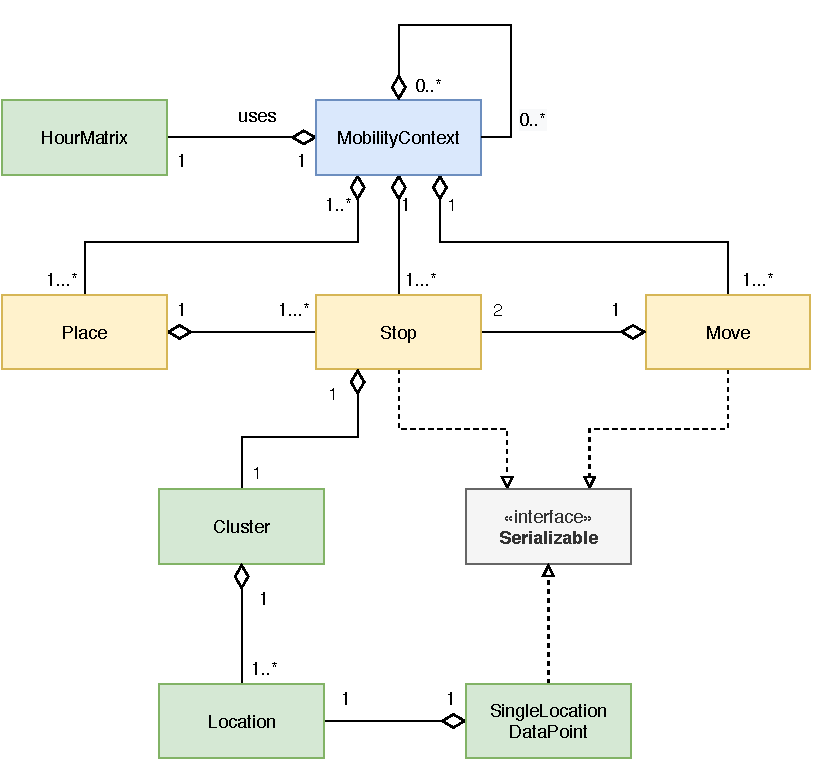
\includegraphics[width=0.7\textwidth]{./images/uml-mobility.pdf}
    \caption{UML diagram for the classes used in the \textit{Mobility Features Package}}
    \label{fig:my_label}
\end{figure}


